\documentclass{standalone}
\usepackage{tikz}
\usetikzlibrary{patterns, positioning}


\begin{document}
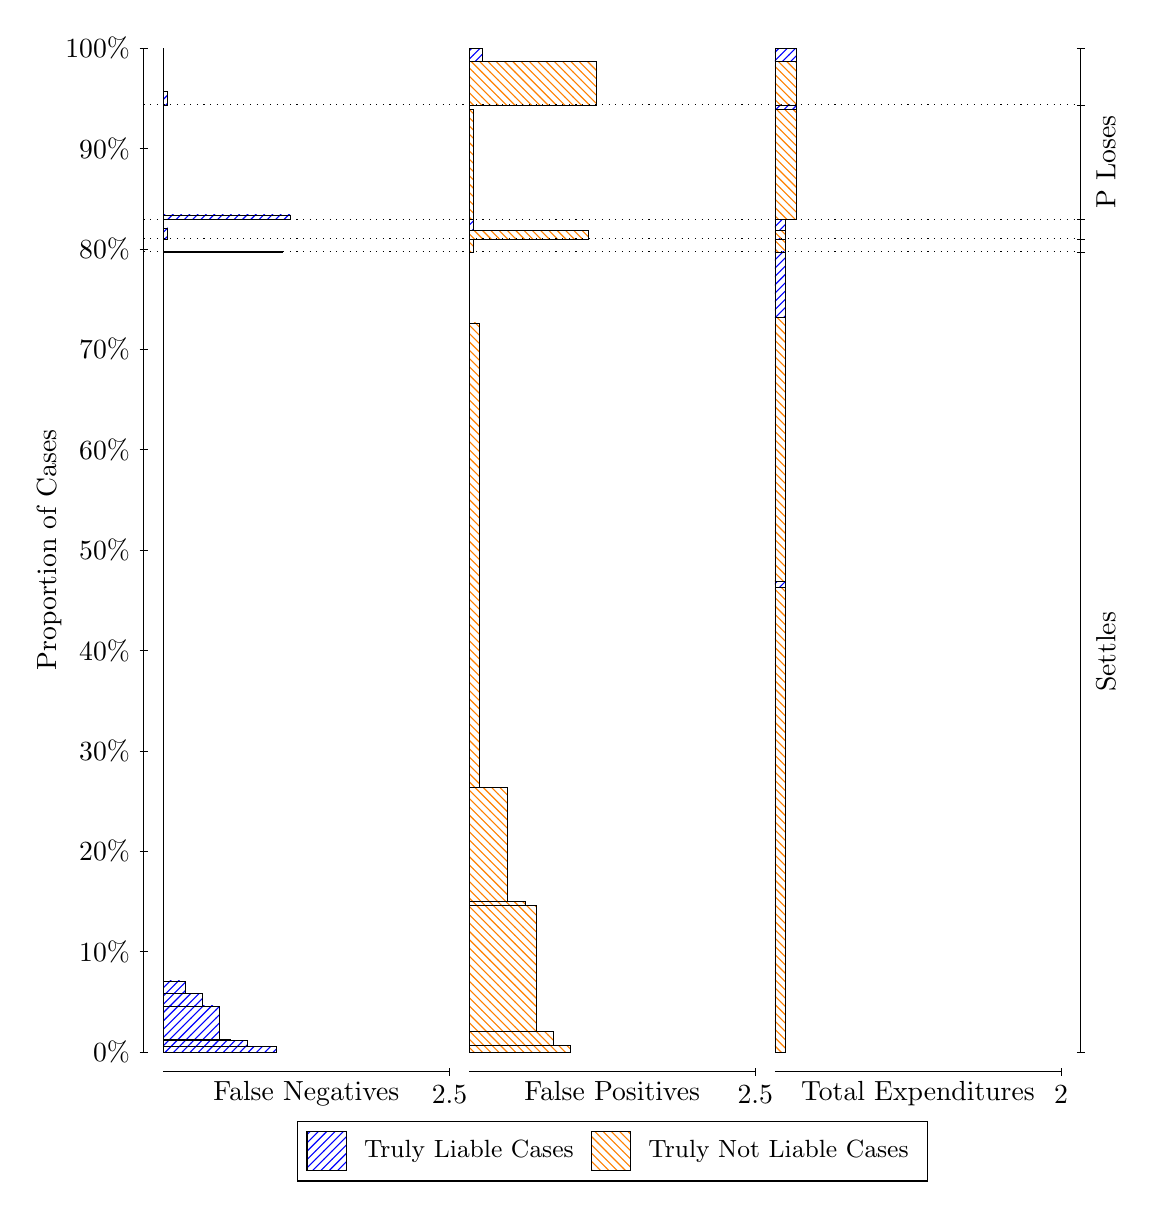
\begin{tikzpicture}
\draw[black, very thin] (1.5,1.75) -- (1.5,14.5);
\node[rotate=90, text=black, anchor=center] at (0.3, 8.125) {Proportion of Cases};
\draw[black, very thin] (1.45,1.75) -- (1.55,1.75);
\node[text=black, anchor=east] at (1.45, 1.75) {0\%};
\draw[black, very thin] (1.45,3.025) -- (1.55,3.025);
\node[text=black, anchor=east] at (1.45, 3.025) {10\%};
\draw[black, very thin] (1.45,4.3) -- (1.55,4.3);
\node[text=black, anchor=east] at (1.45, 4.3) {20\%};
\draw[black, very thin] (1.45,5.575) -- (1.55,5.575);
\node[text=black, anchor=east] at (1.45, 5.575) {30\%};
\draw[black, very thin] (1.45,6.85) -- (1.55,6.85);
\node[text=black, anchor=east] at (1.45, 6.85) {40\%};
\draw[black, very thin] (1.45,8.125) -- (1.55,8.125);
\node[text=black, anchor=east] at (1.45, 8.125) {50\%};
\draw[black, very thin] (1.45,9.4) -- (1.55,9.4);
\node[text=black, anchor=east] at (1.45, 9.4) {60\%};
\draw[black, very thin] (1.45,10.675) -- (1.55,10.675);
\node[text=black, anchor=east] at (1.45, 10.675) {70\%};
\draw[black, very thin] (1.45,11.95) -- (1.55,11.95);
\node[text=black, anchor=east] at (1.45, 11.95) {80\%};
\draw[black, very thin] (1.45,13.225) -- (1.55,13.225);
\node[text=black, anchor=east] at (1.45, 13.225) {90\%};
\draw[black, very thin] (1.45,14.5) -- (1.55,14.5);
\node[text=black, anchor=east] at (1.45, 14.5) {100\%};

\draw[black, very thin] (13.4,1.75) -- (13.4,14.5);
\draw[black, very thin] (13.35,1.75) -- (13.45,1.75);
\node[anchor=west] at (13.35, 1.75) {};
\draw[black, very thin] (13.35,11.911) -- (13.45,11.911);
\node[anchor=west] at (13.35, 11.911) {};
\draw[black, very thin] (13.35,12.077) -- (13.45,12.077);
\node[anchor=west] at (13.35, 12.077) {};
\draw[black, very thin] (13.35,12.321) -- (13.45,12.321);
\node[anchor=west] at (13.35, 12.321) {};
\draw[black, very thin] (13.35,13.778) -- (13.45,13.778);
\node[anchor=west] at (13.35, 13.778) {};
\draw[black, very thin] (13.35,14.5) -- (13.45,14.5);
\node[anchor=west] at (13.35, 14.5) {};

\draw[black, very thin, pattern color=blue, pattern=north east lines] (1.75,1.75) rectangle (3.1852,1.8256);
\draw[black, very thin, pattern color=blue, pattern=north east lines] (1.75,1.8256) rectangle (2.8218,1.9018);
\draw[black, very thin, pattern color=blue, pattern=north east lines] (1.75,1.9018) rectangle (2.6038,1.9112);
\draw[black, very thin, pattern color=blue, pattern=north east lines] (1.75,1.9112) rectangle (2.4585,2.3365);
\draw[black, very thin, pattern color=blue, pattern=north east lines] (1.75,2.3365) rectangle (2.2405,2.4943);
\draw[black, very thin, pattern color=blue, pattern=north east lines] (1.75,2.4943) rectangle (2.0225,2.6522);
\draw[black, very thin, pattern color=orange, pattern=north west lines] (1.75,2.6522) rectangle (1.75,11.911);
\draw[black, very thin, pattern color=blue, pattern=north east lines] (1.75,11.911) rectangle (3.2578,11.915);
\draw[black, very thin, pattern color=orange, pattern=north west lines] (1.75,11.915) rectangle (1.75,12.077);
\draw[black, very thin, pattern color=blue, pattern=north east lines] (1.75,12.077) rectangle (1.8045,12.217);
\draw[black, very thin, pattern color=orange, pattern=north west lines] (1.75,12.217) rectangle (1.75,12.321);
\draw[black, very thin, pattern color=blue, pattern=north east lines] (1.75,12.321) rectangle (3.3668,12.382);
\draw[black, very thin, pattern color=orange, pattern=north west lines] (1.75,12.382) rectangle (1.75,13.778);
\draw[black, very thin, pattern color=blue, pattern=north east lines] (1.75,13.778) rectangle (1.8045,13.946);
\draw[black, very thin, pattern color=orange, pattern=north west lines] (1.75,13.946) rectangle (1.75,14.5);
\draw[black, very thin, pattern color=orange, pattern=north west lines] (5.6333,1.75) rectangle (6.9232,1.8353);
\draw[black, very thin, pattern color=orange, pattern=north west lines] (5.6333,1.8353) rectangle (6.7052,2.0152);
\draw[black, very thin, pattern color=orange, pattern=north west lines] (5.6333,2.0152) rectangle (6.4872,3.6165);
\draw[black, very thin, pattern color=orange, pattern=north west lines] (5.6333,3.6165) rectangle (6.3418,3.658);
\draw[black, very thin, pattern color=orange, pattern=north west lines] (5.6333,3.658) rectangle (6.1238,5.1077);
\draw[black, very thin, pattern color=orange, pattern=north west lines] (5.6333,5.1077) rectangle (5.7605,11.009);
\draw[black, very thin, pattern color=blue, pattern=north east lines] (5.6333,11.009) rectangle (5.6333,11.911);
\draw[black, very thin, pattern color=orange, pattern=north west lines] (5.6333,11.911) rectangle (5.6878,12.074);
\draw[black, very thin, pattern color=blue, pattern=north east lines] (5.6333,12.074) rectangle (5.6333,12.077);
\draw[black, very thin, pattern color=orange, pattern=north west lines] (5.6333,12.077) rectangle (7.1412,12.181);
\draw[black, very thin, pattern color=blue, pattern=north east lines] (5.6333,12.181) rectangle (5.6878,12.321);
\draw[black, very thin, pattern color=orange, pattern=north west lines] (5.6333,12.321) rectangle (5.6878,13.716);
\draw[black, very thin, pattern color=blue, pattern=north east lines] (5.6333,13.716) rectangle (5.6333,13.778);
\draw[black, very thin, pattern color=orange, pattern=north west lines] (5.6333,13.778) rectangle (7.2502,14.331);
\draw[black, very thin, pattern color=blue, pattern=north east lines] (5.6333,14.331) rectangle (5.7968,14.5);
\draw[black, very thin, pattern color=orange, pattern=north west lines] (9.5167,1.75) rectangle (9.6529,7.6512);
\draw[black, very thin, pattern color=blue, pattern=north east lines] (9.5167,7.6512) rectangle (9.6529,7.7268);
\draw[black, very thin, pattern color=orange, pattern=north west lines] (9.5167,7.7268) rectangle (9.6529,11.084);
\draw[black, very thin, pattern color=blue, pattern=north east lines] (9.5167,11.084) rectangle (9.6529,11.911);
\draw[black, very thin, pattern color=orange, pattern=north west lines] (9.5167,11.911) rectangle (9.6529,12.074);
\draw[black, very thin, pattern color=blue, pattern=north east lines] (9.5167,12.074) rectangle (9.6529,12.077);
\draw[black, very thin, pattern color=orange, pattern=north west lines] (9.5167,12.077) rectangle (9.6529,12.181);
\draw[black, very thin, pattern color=blue, pattern=north east lines] (9.5167,12.181) rectangle (9.6529,12.321);
\draw[black, very thin, pattern color=orange, pattern=north west lines] (9.5167,12.321) rectangle (9.7892,13.716);
\draw[black, very thin, pattern color=blue, pattern=north east lines] (9.5167,13.716) rectangle (9.7892,13.778);
\draw[black, very thin, pattern color=orange, pattern=north west lines] (9.5167,13.778) rectangle (9.7892,14.331);
\draw[black, very thin, pattern color=blue, pattern=north east lines] (9.5167,14.331) rectangle (9.7892,14.5);
\draw[black, dotted] (1.5,11.911) -- (13.4,11.911);
\draw[black, dotted] (1.5,12.077) -- (13.4,12.077);
\draw[black, dotted] (1.5,12.321) -- (13.4,12.321);
\draw[black, dotted] (1.5,13.778) -- (13.4,13.778);
\draw[black, very thin] (1.75,1.5) -- (5.3833,1.5);
\node[text=black, anchor=north] at (3.5667, 1.5) {False Negatives};
\draw[black, very thin] (5.3833,1.45) -- (5.3833,1.55);
\node[text=black, anchor=north] at (5.3833, 1.45) {2.5};

\draw[black, very thin] (5.6333,1.5) -- (9.2667,1.5);
\node[text=black, anchor=north] at (7.45, 1.5) {False Positives};
\draw[black, very thin] (9.2667,1.45) -- (9.2667,1.55);
\node[text=black, anchor=north] at (9.2667, 1.45) {2.5};

\draw[black, very thin] (9.5167,1.5) -- (13.15,1.5);
\node[text=black, anchor=north] at (11.333, 1.5) {Total Expenditures};
\draw[black, very thin] (13.15,1.45) -- (13.15,1.55);
\node[text=black, anchor=north] at (13.15, 1.45) {2};

\node[text=black, centered, rotate=90] at (13.72, 6.8306) {Settles};


\node[text=black, centered, rotate=90] at (13.72, 13.049) {P Loses};


\draw (7.449999999999999,1.5) node[draw=none] (baseCoordinate) {};
\begin{scope}[align=center]
        \matrix[scale=0.5, draw=black, below=0.5cm of baseCoordinate, nodes={draw}, column sep=0.1cm]{
            \node[rectangle, draw, minimum width=0.5cm, minimum height=0.5cm, pattern color=blue, pattern=north east lines] {}; &
            \node[draw=none, font=\small, text=black] (B) {Truly Liable Cases}; &
            \node[rectangle, draw, minimum width=0.5cm, minimum height=0.5cm, pattern color=orange, pattern=north west lines] {}; &
            \node[draw=none, font=\small, text=black] (B) {Truly Not Liable Cases}; \\
            };
\end{scope}

\end{tikzpicture}
\end{document}